\documentclass[conference]{IEEEtran} % LaTeX2e
\usepackage[noadjust]{cite}
\usepackage{amssymb,amsmath,graphicx,float,array}

\newcommand\real{\mathbb{R}}

\begin{document}

\title{Model Predictive Control of a Mobile Robot Using Linearization}

\author{\authorblockN{Felipe K\"{u}hne \qquad Walter Fetter Lages \qquad Jo\~{a}o Manoel Gomes da Silva Jr.}
\authorblockA{Federal University of Rio Grande do Sul\\
Electrical Engineering Department\\
Av. Oswaldo Aranha, 103\\
Porto Alegre, RS 90035-190 Brazil\\
Email: \{kuhne,fetter,jmgomes\}@eletro.ufrgs.br}
%\and
%\authorblockN{Walter Fetter Lages}
%\authorblockA{Federal University of Rio Grande do Sul\\
%Electrical Engineering Department\\
%Av. Oswaldo Aranha, 103\\
%Porto Alegre, RS 90035-190 Brazil\\
%Email: fetter@eletro.ufrgs.br}
%\and
%\authorblockN{Jo\~{a}o Manoel Gomes da Silva Jr.}
%\authorblockA{Federal University of Rio Grande do Sul\\
%Electrical Engineering Department\\
%Av. Oswaldo Aranha, 103\\
%Porto Alegre, RS 90035-190 Brazil\\
%Email: jmgomes@eletro.ufrgs.br}
}

\maketitle

\begin{abstract}
This paper presents an optimal control scheme for a wheeled mobile robot (WMR) with nonholonomic constraints. It is well known that a WMR with nonholonomic constraints can not be feedback stabilized through continuously differentiable, time-invariant control laws. By using model predictive control (MPC), a discontinuous control law is naturally obtained. One of the main advantages of MPC is the ability to handle constraints (due to state or input limitations) in a straightforward way. Quadratic programming (QP) is used to solve a linear MPC by successive linearization of an error model of the WMR. Simulation and experimental results are shown.
\end{abstract}
%\begin{keywords}
%Wheeled mobile robots, model predictive control, trajectory tracking.
%\end{keywords}
%\thispagestyle{empty}\pagestyle{empty}

\section{Introduction}
\label{sec:intro}

The field of mobile robot control has been the focus of great research
effort in the past decades. Despite the apparent simplicity of the kinematic
model of a wheeled mobile robot (WMR), the existence of nonholonomic
constraints turns the design of stabilizing control laws for those systems
in a considerable challenge. Due to Brockett conditions~\cite{brockett82}, a
continuously differentiable, time-invariant stabilizing feedback control law
can not be obtained. To overcome these limitations most works uses
non-smooth and time-varying control
laws~\cite{bloch89,samson91,canudas92,yamamoto94,murray97}. Recent works
dealing with robust and adaptive control of WMRs can be found in
\cite{oya03,dixon04}.

However, in realistic implementations it is difficult to obtain good
performance, due to the constraints on inputs or states that naturally
arise. None of the previously cited works have taken those constraints
into account. This can be done in a straightforward way by using model
predictive control (MPC) schemes. For a WMR this is an important issue,
since the position of the robot can be restricted to belong to a safe
region of operation. By considering input constraints, control actions that
respect actuators limits can be generated. 

{\bf Besides these possibilities, coordinate transformations of the dynamic system to {\em chained} or {\em power} forms~\cite{bloch89}, as made for non-smooth and time-varying control schemes, are not necessary anymore, which turns the choice of tuning parameters for the MPC more intuitive. Regarding the nonholonomic features of the WMR, a piecewise-continuous (non-smooth) control law, with MPC, is implicitly generated.}

Model predictive control is an {\bf open-loop, optimal} control strategy that uses the model of the
system to obtain an optimal control sequence by minimizing an objective
function. At each sampling interval, the model is used to predict the behavior of the system over a prediction horizon. Based on these predictions, an objective
function is minimized with respect to the future sequence of inputs{\bf , thus requiring the solution of a constrained optimization problem for each sampling interval}. Although prediction and optimization are performed over a future
horizon, only the values of the inputs for the current sampling interval are
used and the same procedure is repeated at the next sampling time. This
mechanism is known as {\it moving} or {\it receding horizon} strategy, in
reference to the way in which the time window shifts forward from one sampling time
to the next one.

For complex, constrained, multivariable control problems, MPC has become an
accepted standard in the process industries~\cite{bemporad02}. It is used in
many cases, where plants being controlled are sufficiently {\em slow} to
allow its implementation~\cite{mayne00}. However, for systems with fast
and/or nonlinear dynamics, the implementation of such
technique remains fundamentally limited in applicability, due to large
amount of {\em on-line} computation required~\cite{cannon00}.

{\bf The dynamic description of a WMR requires the use of nonlinear system models. Although nonlinear model predictive control (NMPC) has been well developed regarding its theoretical aspects~\cite{mayne00,chen98}, the computational effort necessary is much greater in comparison to the linear version, since now there is a nonlinear programming problem to be solved on-line, which is nonconvex, has a larger number of decision variables and a global minimum is in general impossible to find~\cite{henson98}. In this paper, we propose a strategy in order to overcome at least part of these problems. The fundamental idea consists in using a successive linearization approach, as briefly outlined in~\cite{henson98}, yielding a linear, time-varying description of the system beeing solved through linear MPC. Then, considering the control inputs as the decision variables, it is possible to transform the optimization problem in a Quadratic programming (QP) problem. The advantage is that existing QP solvers are fast, extremely robust numerically and gives always the global optimal solution.} It is then shown that even a real-time implementation is possible.
Although MPC is not a new control method, works dealing with MPC of WMRs are
recent and sparse~\cite{ollero91,rico99,essen01}.

The remainder of this paper is organized as follows: in the next section the
kinematic model of the WMR is shown. The MPC algorithm is depicted in
section~\ref{sec:mpc}. Simulation results in {\sc Matlab} are shown in
section~\ref{sec:simulations}, where an eight-like trajectory is used as
reference. Section~\ref{sec:exp} presents some considerations regarding real-time implementation.


\section{Kinematic Model of the WMR}
\label{sec:model}

In this section the kinematic model of the WMR is described. A mobile robot
made up of a rigid body and non deforming wheels is considered (see
Fig.~\ref{fig:robot}). It is assumed that the vehicle moves on a plane
without slipping, i.e., there is a pure rolling contact between the wheels
and the ground. The kinematic model of the WMR used here is given
by~\cite{Campion:TRA-12-1}:

\begin{equation}
\label{eqn:model}
	\left\{
		\begin{aligned}
			\dot x	  &= v\cos\theta \\
			\dot y	  &= v\sin\theta \\
			\dot \theta &= w
		\end{aligned}
	\right.
\end{equation}
or, in a more compact form as
\begin{equation}
\label{eqn:modelshort}
	\dot{\bf x} = f({\bf x},{\bf u}),	
\end{equation}
\noindent where ${\bf x}\triangleq[x~~y~~\theta]^T$ describes the
configuration (position and orientation) of the center of the axis of the
wheels, $C$, with respect to a global inertial frame $\{O,X,Y\}$.
${\bf u}\triangleq[v~~w]^T$ is the control input, where $v$ and $w$ are the
linear and the angular velocities, respectively.

\begin{figure}[b]
	\centering
	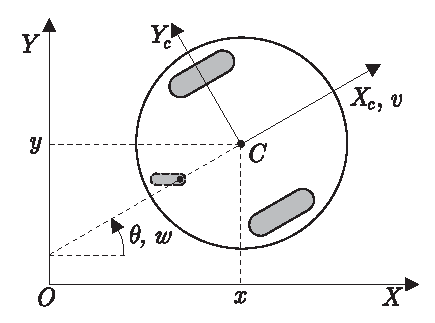
\includegraphics[width=0.67\linewidth]{Figures/robot.eps}
	\caption{Coordinate system of the WMR.}
	\label{fig:robot}
\end{figure}

{\bf A linear model is obtained by computing an error model with respect to a reference car. To do so, consider a reference car described by the same model (\ref{eqn:modelshort}) as the robot. Hence, its trajectory ${\bf x}_r$ and ${\bf u}_r$ is related by:
\begin{equation}
	\dot{\bf x}_r=f({\bf x}_r,{\bf u}_r)
\label{eqn:referencecar}
\end{equation}

By expanding the right side of (\ref{eqn:modelshort}) in Taylor series around the point $({\bf x}_r,{\bf u}_r)$ and discarding the high order terms it follows that
\begin{equation}
\label{eqn:taylor}
	\dot{\bf x} = f({\bf x}_r,{\bf u}_r) + f_{{\bf x},r}({\bf x}-{\bf x}_r) + f_{{\bf u},r}({\bf u}-{\bf u}_r),
\end{equation}
where $f_{{\bf x},r}$ and $f_{{\bf u},r}$ are the jacobians of $f$ with respect to ${\bf x}$ and ${\bf u}$, respectively, evaluated around the reference point $({\bf x}_r,{\bf u}_r)$.

Then, the subtraction of~(\ref{eqn:referencecar}) from~(\ref{eqn:taylor}) results in:
\begin{equation}
\label{eqn:conterror}
	{\dot{\tilde{\bf x}}} = f_{{\bf x},r}\tilde{\bf x}+f_{{\bf u},r}\tilde{\bf u}
\end{equation}

Hence, $\tilde{\bf x}\triangleq{\bf x}-{\bf x}_r$ represents the
error with respect to the reference car and $\tilde{\bf u}\triangleq
{\bf u}-{\bf u}_r$ is its associated perturbation control input.

The approximation of $\dot{\bf x}$ by using forward differences gives the following discrete-time model system:

\begin{equation}
\label{eqn:error}
	\tilde{\bf x}(k+1) = {\bf A}(k)\tilde{\bf x}(k)+{\bf B}(k)\tilde{\bf u}(k),
\end{equation}

\noindent with

\begin{align*}
	{\bf A}(k) &\triangleq \begin{bmatrix}
		1 & 0 & -v_r(k)\sin\theta_r(k)T \\
		0 & 1 &  v_r(k)\cos\theta_r(k)T \\
		0 & 0 & 1
	\end{bmatrix} \\
	{\bf B}(k) &\triangleq \begin{bmatrix}
		\cos\theta_r(k)T & 0 \\
		\sin\theta_r(k)T & 0 \\
		0 			  & T
	\end{bmatrix}
\end{align*}
where $T$ is the sampling period and $k$ is the sampling time. }

Indeed, the convergence of ${\bf x}$ to ${\bf x}_r$ is equivalent to the
convergence of $\tilde{\bf x}$ to the set ${\cal O}=\{{\bf x}|(\tilde
x,\tilde y,\tilde\theta)=(0,0,2\pi n)\},n\in \{0,\pm1,\pm2,\ldots\}$.

In~\cite{bloch89} it is shown that the nonlinear, nonholonomic system
(\ref{eqn:model}) is fully controllable, i.e., it can be steered from any
initial state to any final state in finite time by using finite inputs. It
is easy to see that when the robot is not moving, the linearization about a
stationary operating point is not controllable. However, this linearization
becomes controllable as long as the control input ${\bf u}$ is not
zero~\cite{samson91}. This implies the tracking of a reference trajectory
being possible with linear MPC~\cite{essen01}.


\section{The MPC Algorithm}
\label{sec:mpc}

It was said in section~\ref{sec:intro} that the essence of a MPC scheme is
to optimize predictions of process behavior over a sequence of future control inputs. Such
a prediction is accomplished by using a process model over a finite time
interval, called the {\em prediction horizon}. At each sampling time, the
model predictive controller generates an optimal control sequence by solving
an optimization problem. The first element of this sequence is applied to the
plant. The problem is solved again at the next sampling time using the
updated process measurements and a shifted horizon.

For the sake of simplicity, we assume in this work that the states of the
plant are always available for measurement and that there are no plant/model
mismatch.

The objective function to be minimized can be stated as a quadratic function of
the states and control inputs:

\begin{multline}
\label{eqn:cost}
	\Phi(k) = \sum_{j=1}^{N}\tilde{\bf x}^T(k+j|k){\bf Q}\tilde{\bf x}(k+j|k) + \\ + \tilde{\bf u}^T(k+j-1|k){\bf R}\tilde{\bf u}(k+j-1|k),
\end{multline}

\noindent where $N$ is the prediction horizon and ${\bf Q}$, ${\bf R}$ are
weighting matrices, with ${\bf Q}\geq 0$ and ${\bf R}>0$. The notation
$a(m|n)$ indicates the value of $a$ at the instant $m$ predicted at instant
$n$.

{\bf 
Hence, the optimization problem can be stated as to find $\tilde{\bf
u}^\star$ such that:

\begin{equation}
\label{eqn:optim}
	\tilde{\bf u}^\star = \arg\min_{\tilde{\bf u}}\left\{\Phi(k)\right\}
\end{equation}
\noindent s. a.
\begin{align}
	{\bf C\tilde x} &\leq {\bf c} \label{eqn:restx} \tag{\ref{eqn:optim}a} \\
	{\bf D\tilde u} &\leq {\bf d} \label{eqn:restu} \tag{\ref{eqn:optim}b}
\end{align}

\noindent where $\Phi(k)$ is the {\em objective function} and $\tilde{\bf u}$ is the
free variable in the optimization. Eqs. (\ref{eqn:restx}) and (\ref{eqn:restu}) are a general way to describe constraints in the state and control variables, respectively. When there are amplitude constraints, we have
\begin{equation*}
	\begin{bmatrix} {\bf I} \\ -{\bf I} \end{bmatrix} \tilde{\bf u} \leq \begin{bmatrix} \tilde{\bf u}_{max} \\ -\tilde{\bf u}_{min} \end{bmatrix}, \quad \begin{bmatrix} {\bf I} \\ -{\bf I} \end{bmatrix} \tilde{\bf x} \leq \begin{bmatrix} \tilde{\bf x}_{max} \\ -\tilde{\bf x}_{min} \end{bmatrix},
\end{equation*}
which turns out that
\begin{align*}
	\tilde{\bf u}_{min} \leq \tilde{\bf u} \leq \tilde{\bf u}_{max}, \\
	\tilde{\bf x}_{min} \leq \tilde{\bf x} \leq \tilde{\bf x}_{max},
\end{align*}
where the subscripts $min$ and $max$ stands for lower and upper bounds, respectively. Also, constraints in the rate of change of control and states can be formulated in the same way. Here we will only consider constraints in the amplitude of the control input. }

The problem of minimizing (\ref{eqn:cost}) is solved at each time step $k$,
yielding a sequence of optimal control $\{\tilde{\bf
u}^\star(k|k),\cdots,\tilde{\bf u}^\star(k+N-1|k)\}$ and the optimal cost
$\Phi^\star(k)$. The MPC control law is implicitly given by the first
control action of the sequence of optimal control, $\tilde{\bf u}^\star(k|k)$. A
block diagram with all components of the system is shown in Fig.
\ref{fig:bloco}, where the indexes $(k|k)$ are omitted.

\begin{figure}[b]
	\centering
	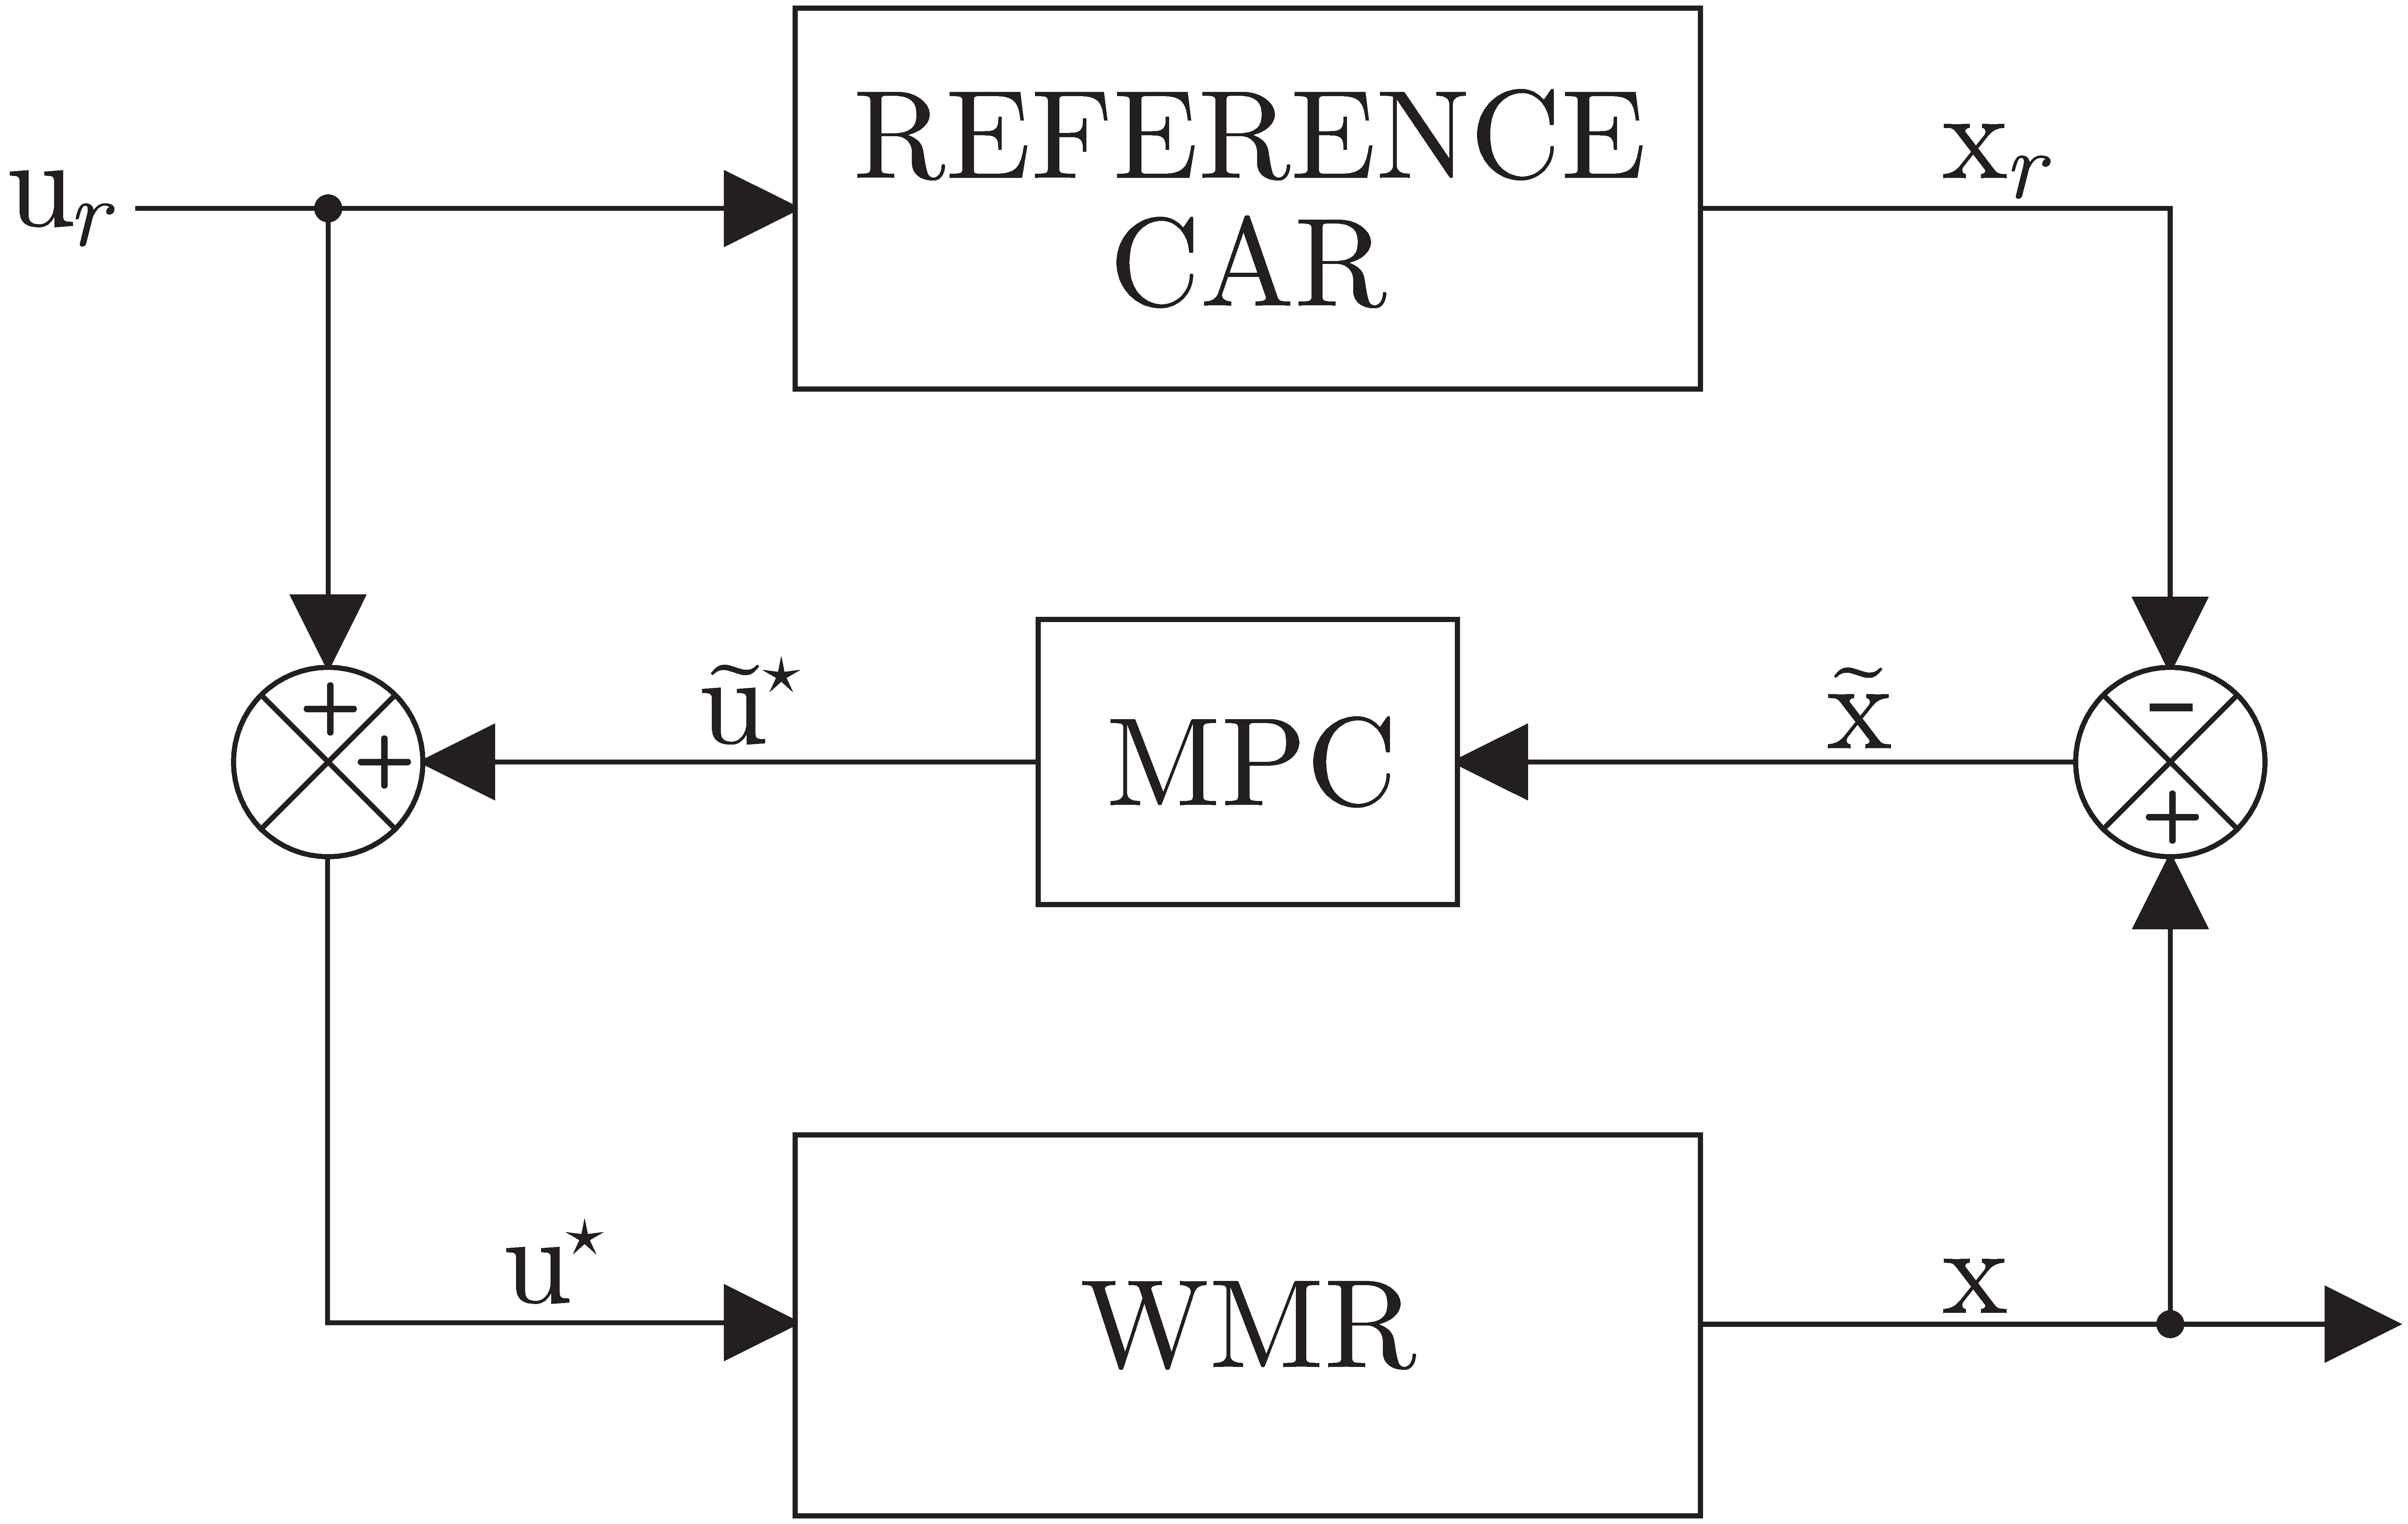
\includegraphics[width=.84\linewidth]{Figures/bloco.eps}
	\caption{Block diagram of the system.}
	\label{fig:bloco}
\end{figure}

To formulate the optimization problem in a usual Quadratic Programming form, we introduce the
following vectors:
\begin{equation*}
	\bar{\bf x}(k+1) \triangleq \begin{bmatrix}
		\tilde{\bf x}(k+1|k) \\ \tilde{\bf x}(k+2|k) \\ \vdots \\ \tilde{\bf x}(k+N|k) 
	\end{bmatrix} \quad
	\bar{\bf u}(k) \triangleq \begin{bmatrix}
		\tilde{\bf u}(k|k)  \\ \tilde{\bf u}(k+1|k) \\ \vdots \\ \tilde{\bf u}(k+N-1|k)
	\end{bmatrix}
\end{equation*}

Thus, (\ref{eqn:cost}) can be rewritten as:
\begin{equation}\label{eqn:cost2}
	\Phi(k) = \bar{\bf x}^T(k+1)\bar{\bf Q}\bar{\bf x}(k+1) + \bar{\bf u}^T(k)\bar{\bf R}\bar{\bf u}(k),
\end{equation}
with
\begin{equation*}
	\bar {\bf Q} \triangleq \begin{bmatrix}
		{\bf Q} & {\bf 0} & \cdots & {\bf 0} \\
		{\bf 0} & {\bf Q} & \cdots & {\bf 0} \\
		\vdots  & \vdots  & \ddots & \vdots  \\
		{\bf 0} & {\bf 0} & \cdots & {\bf Q}
	\end{bmatrix} \quad
	\bar {\bf R} \triangleq \begin{bmatrix}
		{\bf R} & {\bf 0} & \cdots & {\bf 0} \\
		{\bf 0} & {\bf R} & \cdots & {\bf 0} \\
		\vdots  & \vdots  & \ddots & \vdots  \\
		{\bf 0} & {\bf 0} & \cdots & {\bf R}
	\end{bmatrix}
\end{equation*}

Therefore, it is possible from~(\ref{eqn:error}) to write $\bar{\bf x}(k+1)$ as:
\begin{equation}\label{eqn:exbar}
	\bar{\bf x}(k+1) = \bar{\bf A}(k)\tilde{\bf x}(k|k)+\bar{\bf B}(k)\bar{\bf u}(k),
\end{equation}
with
\begin{equation*}
	\bar{\bf A}(k) \triangleq \begin{bmatrix}
		{\bf A}(k|k) \\ {\bf A}(k|k){\bf A}(k+1|k) \\ \vdots \\ \alpha(k,0)
	\end{bmatrix}
\end{equation*}
{\small
\begin{multline*}
		\bar{\bf B}(k) \triangleq \\ \begin{bmatrix}
			{\bf B}(k|k)		       & {\bf 0} 			    	 & \cdots & {\bf 0}         \\
			{\bf A}(k+1|k){\bf B}(k|k) & {\bf B}(k+1|k)      	 & \cdots & {\bf 0}         \\
			\vdots			       & \vdots				 & \ddots & \vdots          \\
			\alpha(k,1){\bf B}(k|k)    & \alpha(k,2){\bf B}(k+1|k) & \cdots & {\bf B}(k+N-1|k)
		\end{bmatrix}
\end{multline*}
}
where  $\alpha(k,j)$ is defined as:
\begin{equation*}
	\alpha(k,j) \triangleq \prod_{i=j}^{N-1}{\bf A}(k+i|k),
\end{equation*}

From (\ref{eqn:cost2}) and (\ref{eqn:exbar}), we can rewrite the objective function (\ref{eqn:cost}) in a standard quadratic form:
\begin{equation*}
	\Phi(k) = \frac{1}{2}\bar{\bf u}^T(k){\bf H}(k)\bar{\bf u}(k) + {\bf f}^T(k)\bar{\bf u}(k) + {\bf d}(k)
\end{equation*}
with
\begin{align*}
	{\bf H}(k) &\triangleq 2\left(\bar{\bf B}(k)^T(k)\bar{\bf Q}\bar{\bf B}(k)+\bar{\bf R}\right) \\
	{\bf f}(k) &\triangleq 2\bar{\bf B}^T(k)\bar{\bf Q}\bar{\bf A}(k)\tilde{\bf x}(k|k) \\
	{\bf d}(k) &\triangleq \tilde{\bf x}^T(k|k)\bar{\bf A}^T(k)\bar{\bf Q}\bar{\bf A}(k)\tilde{\bf x}(k|k)
\end{align*}

The matrix ${\bf H}$ is a {\em Hessian} matrix, and must be positive
definite. It describes the quadratic part of the objective function, and the
vector ${\bf f}$ describes the linear part. $\bf d$ is independent of
$\tilde{\bf u}$ and does not matter for the determination of $\bf u^\star$.

Model predictive control is based on the assumption that for a small time
horizon plant and model behavior are the same. For this assumption to hold
the plant/model mismatch should be kept small. Obviously, for any real
world plant, control inputs are subject to physical limitations. Hence, to
avoid large plant/model mismatch those limitations should be considered
while computing control inputs. This can be done in a straightforward way by
defining upper and lower bounds on the control input. The optimization
problem must then be solved while ensuring that the control will remain
between certain lower and upper bounds. Hence, the following control
constraint can be written:

\begin{equation}\label{eqn:uconstr}
	{\bf u}_{min}(k) \leq {\bf u}(k) \leq {\bf u}_{max}(k),
\end{equation}

Since the free variable in the optimization is $\tilde{\bf u}(k)$,
the constraint (\ref{eqn:uconstr}) must be rewritten with respect to this
variable:

\begin{equation*}
	{\bf u}_{min}(k) - {\bf u}_r(k) \leq \tilde{\bf u}(k) \leq {\bf u}_{max}(k) - {\bf u}_r(k),
\end{equation*}
or, in the vector form,
\begin{equation*}
	\bar{\bf u}_{min}(k) - \bar{\bf u}_r(k) \leq \bar{\bf u}(k) \leq \bar{\bf u}_{max}(k) - \bar{\bf u}_r(k)
\end{equation*}
\noindent with
\begin{align*}
	\bar{\bf u}_{min}(k) &\triangleq \begin{bmatrix}
		{\bf u}_{min}(k) \\ {\bf u}_{min}(k+1) \\ \vdots \\ {\bf u}_{min}(k+N-1)
	\end{bmatrix} \\
	\bar{\bf u}_{max}(k) &\triangleq \begin{bmatrix}
		{\bf u}_{max}(k) \\ {\bf u}_{max}(k+1) \\ \vdots \\ {\bf u}_{max}(k+N-1)
	\end{bmatrix} \\
	\bar{\bf u}_r(k) &\triangleq \begin{bmatrix}
		{\bf u}_r(k) \\ {\bf u}_r(k+1) \\ \vdots \\ {\bf u}_r(k+N-1)
	\end{bmatrix}
\end{align*}


\section{Simulation results}
\label{sec:simulations}

In this section, simulation results are shown for the MPC applied to the
WMR. The optimization problem has been solved with the {\sc Matlab} routine
{\tt quadprog}. The initial configuration of the WMR and the reference car
are, respectively, ${\bf x}(0)=[0~~-1~~\pi/2]^T$ and ${\bf
x}_r(0)=[0~~0~~0]^T$. The weighting matrices used are ${\bf
Q}=diag(1,1,0.5)$ and ${\bf R}=0.1{\bf I}_{2\times 2}$. The prediction
horizon is $N=5$. Constraints in the amplitude of the control variables
are: $v_{min}=-0.4 m/s$, $v_{max}=0.4 m/s$, $w_{min}=-0.4 rad/s$ and
$w_{max}=0.4 rad/s$.

\begin{figure}[htbp]
	\centering
    \includegraphics[width=.99\linewidth]{Figures/traj8.eps}
    \caption{Trajectory in the $XY$ plane.}
    \label{fig:traj8}
\end{figure}
\begin{figure}
	\centering
    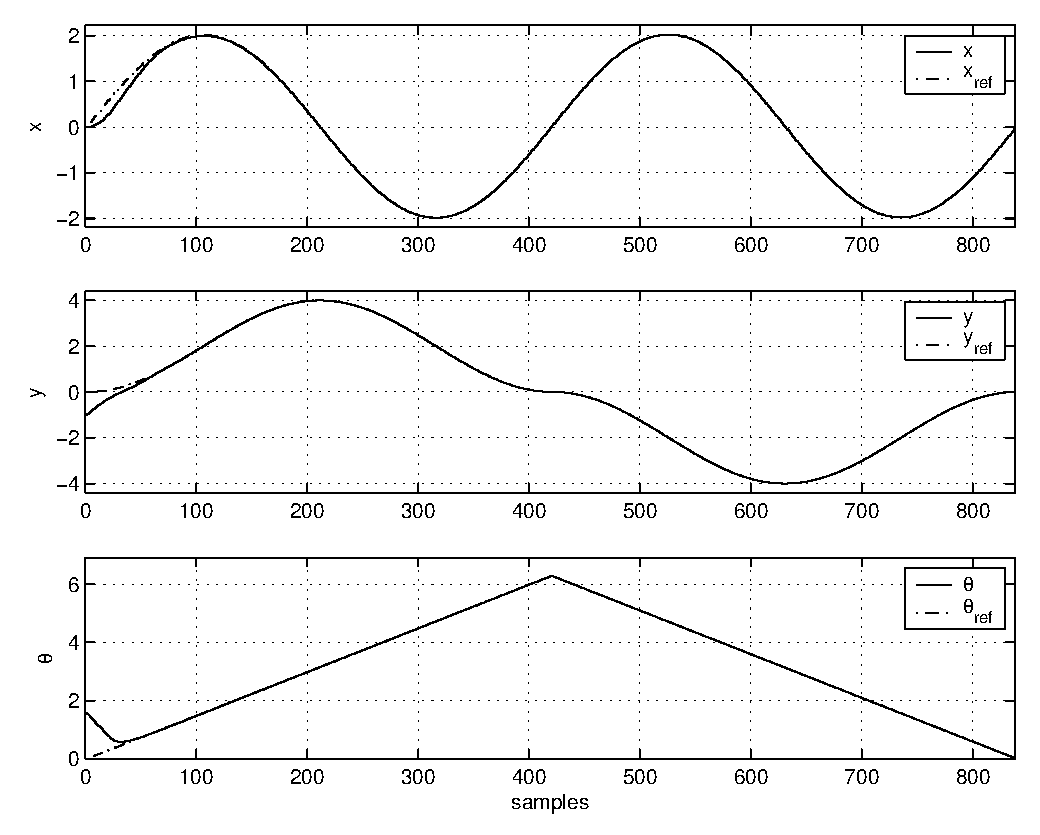
\includegraphics[width=.99\linewidth]{Figures/states.eps}
    \caption{States $x$, $y$ and $\theta$.}
    \label{fig:states}
\end{figure}

It can be clearly seen that the state asymptotically converges to the
reference. In Fig.~\ref{fig:traj8} and \ref{fig:states}, the dash-dotted
line stands for the reference trajectory.
Fig.~\ref{fig:errors} shows the errors of the states converging to zero. It
must be noted that, even without error in the $x$ state, the WMR must turn
away from the reference trajectory to obey the nonholonomic constraint. In
Fig.~\ref{fig:controls}, it can be seen that the control inputs are inside
the limits imposed by the constraints. Since the state and control errors
converge to zero (Fig.~\ref{fig:errors}), one could say that the value of
the objective function should also converges to zero. This fact can be observed in
Fig.~\ref{fig:cost}.

\begin{figure}[htbp]
	\centering
    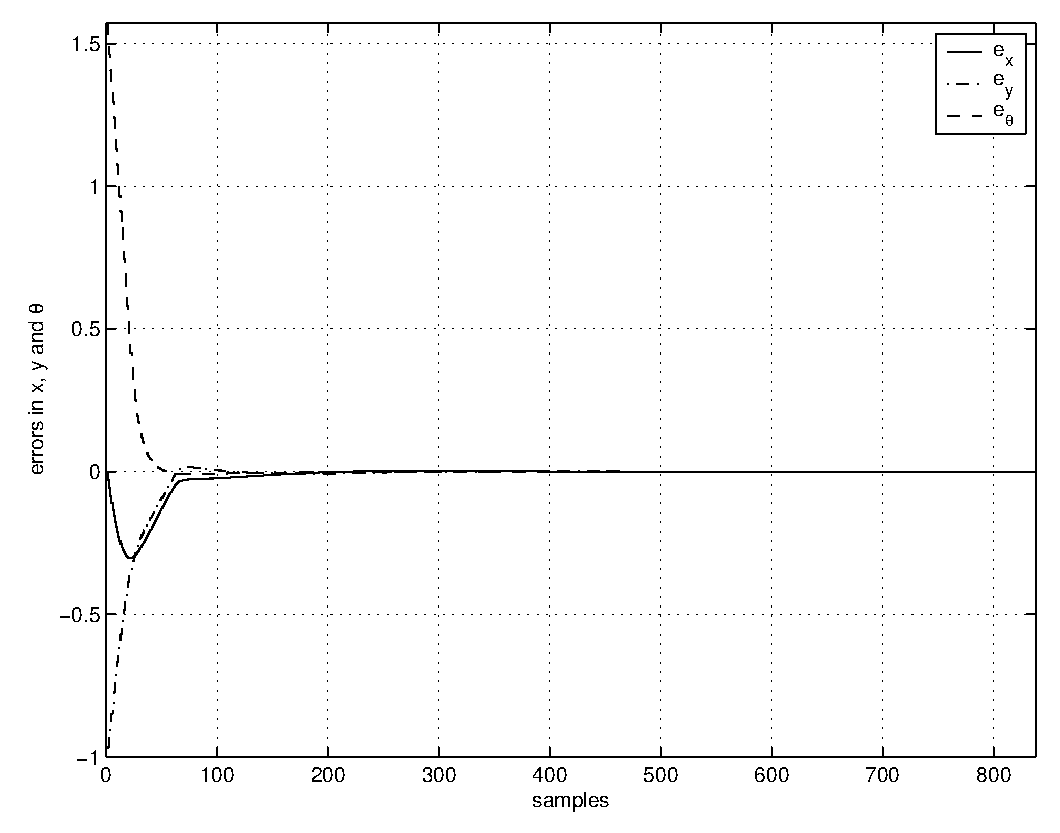
\includegraphics[width=.99\linewidth]{Figures/errors.eps}
    \caption{Errors.}
    \label{fig:errors}
\end{figure}

\begin{figure}[htbp]
	\centering
    \includegraphics[width=.99\linewidth]{Figures/controls.eps}
    \caption{Controls bounded by the constraints.}
    \label{fig:controls}
\end{figure}

\begin{figure}[htbp]
	\centering
    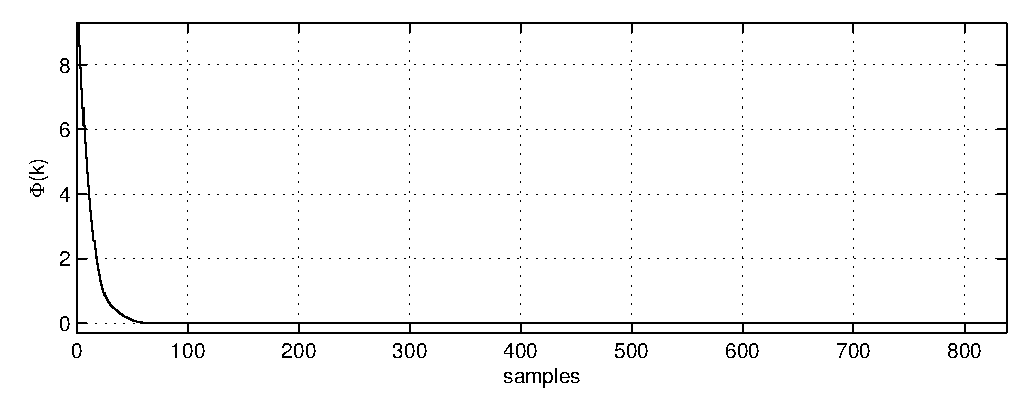
\includegraphics[width=.99\linewidth]{Figures/cost.eps}
    \caption{Objective function $\Phi(k)$.}
    \label{fig:cost}
\end{figure}

A typical measure of convergence is the integrated error~\cite{essen01},

\begin{equation*}
	\varepsilon \triangleq \frac{1}{K_f}\sum_{k=0}^{K_f}\left\|\tilde{\bf x}\right\|^2,
\end{equation*}

\noindent where $K_f$ is the number of steps to cover all the trajectory and
$\left\|{\bf\cdot}\right\|$ is the euclidian norm.

Table~\ref{table:table1} shows some results relating the computational cost
and the error $\varepsilon$ as a function of the prediction horizon $N$.
The computing time is the mean time to solve the optimization problem
for one step of the trajectory. The number of flops needed to complete the
calculations due at each sampling time is also shown.
 
\begin{table}[htpb]
 \caption{Influence of prediction horizon in computing time and $\varepsilon$}
 \label{table:table1}
 \centering
 \begin{tabular}{cccc}
  \hline
  Horizon & Computing time (s) & Flops & $\varepsilon$ \\
  \hline\hline
  1  & 0.0110 & 4343    & 3.2578  \\
  3  & 0.0114 & 9529    & 1.4384  \\
  5  & 0.0135 & 25643   & 1.3757  \\
  10 & 0.0271 & 160180  & 1.3695  \\
  15 & 0.0582 & 528570  & 1.3798  \\
  20 & 0.1156 & 1269500 & 1.3927  \\
  30 & 0.3402 & 4949000 & 1.4856  \\
  \hline
 \end{tabular}
\end{table}
 
Obviously the prediction horizon must be chosen in a way such that the
computing time is smaller than the sampling period. Here, $T=0.1 s$,
therefore with $N=20$ or above the MPC is not feasible. On the other hand,
by increasing $N$ above $5$ there is not sensible improvement on
$\varepsilon$. Furthermore, for $N=5$ the computing time is approximately seven
times smaller than the sampling period. Hence, five steps ahead is a good
choice for prediction horizon. The computations were carried out on a
computer with an Athlon 2600+ processor running Linux operating system. 
 
\section{Real-time Experiments}
\label{sec:exp}

Figure~\ref{fig:twil} shows the mobile robot developed in our labs and used in
this work. It has a cylindrical geometry with 1.35m in height and 0.30 cm in
radius and uses a differential-drive steering. The software is based on a
real-time variation of the Linux operating system called
RTAI~\cite{Dozio:2003}.

\begin{figure}[htbp]
	\centering
	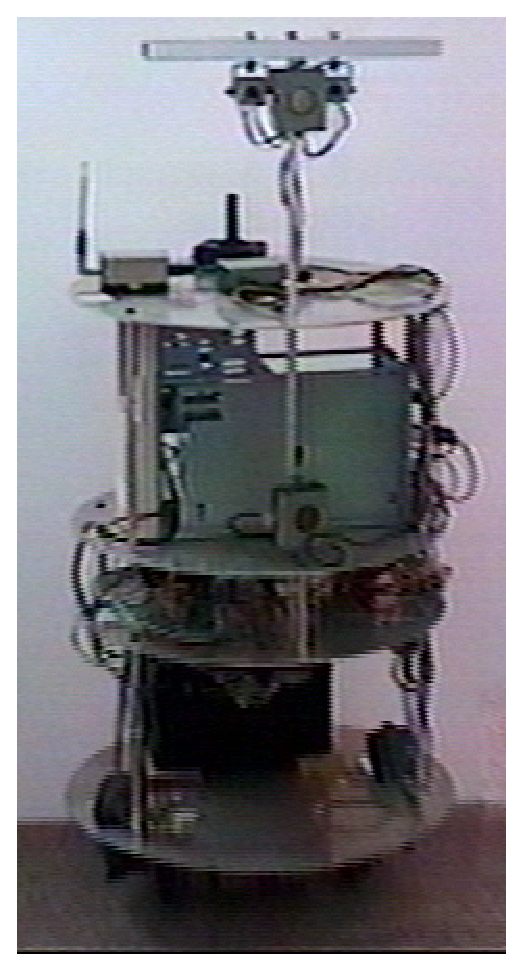
\includegraphics[width=0.65\linewidth]{Figures/twil6.ps}
	\caption{The Twil Mobile Robot.}
	\label{fig:twil}
\end{figure}

The use of MPC for real-time control of systems with fast dynamics such as a
WMR has been hindered for some time due to its numerical intensive
nature~\cite{cannon00}. However, with the development of increasingly faster
processors the use of MPC in demanding applications becomes possible.
Indeed, the data in Table~\ref{table:table1} provides enough evidence that a
standard of the shelf computer is able to run a MPC based controller for a
WMR. An Athlon 2600+ gives an peak performance between 576 and 1100 Mflops
using double precision computations accordingly
to~\cite{aburto:flops-1992-dec}, a de-facto standard for floating point
performance measurement. Therefore, the MPC algorithm proposed here could be
computed for $N=30$ in about 10ms, while the dynamics of the mobile robot
used here is such that sampling periods between 50 and 100 ms are adequate,
revealing that a real-time implementation is plenty possible.


\section{Conclusion}
\label{sec:conclusions}

This paper presented an application of MPC to {\bf the problem of trajectory tracking of} a nonholonomic WMR. The
solution of the optimization problem through a standard QP method was shown.
The obtained control signals were such that the constraints imposed on the
control variables were respected. 

{\bf As shown above, the choice of MPC for the application given here is well justified by some advantages: the straightforward way in which state/input constraints can be handled; coordinate transformations to a chained or power form are not necessary; the MPC implicitly generates a piecewise-continuous control law (which is necessary for nonholonomic systems); the MPC can be casted as an optimal trajectory planning.

It was clearly shown that with a successive linearization approach, the open-loop, optimal control problem was successfully solved, arising the possibility of a real time implementation. With such technique, it was possible the transformation of the optimization problem in a standard QP formulation, which is fast and extremely robust numerically.}


\section*{Acknowledgments}

The authors gratefully acknowledge the financial support from CAPES.

\bibliographystyle{IEEEtran}
\bibliography{mechrob04_v11}

\end{document}
